\chapter{Projet : emploi du temps}

Le but initial du projet ``Emploi du temps'' était de recréer un emploi du temps visuel pour n'importe quel étudiant (ou personnel) de l'UTC, à la manière de celui disponible sur l'ENT\footnote{\url{https://webapplis.utc.fr/edt/index.html}}. Cet emploi du temps se devait d'être un minimum responsive (affichable correctement sur mobile). Par ailleurs, ce projet reposait sur l'utilisation d'une API fournie par l'UTC pour récupérer les emplois du temps au format JSON (voir explications plus bas).

\medskip

\noindent De plus, d'autres objectifs supplémentaires nous ont été donnés:
\begin{itemize}
  \item Pouvoir afficher simultanément plusieurs emplois du temps
  \item Vérifier la disponibilité de l'API de l'UTC
\end{itemize}
En plus de ces objectifs secondaires, nous avons rajouté quelques fonctionnalités, détaillées plus bas.

\section{Choix préliminaires}

Avant de rentrer dans le vif du sujet, il est important de préciser comment nous avons pensé notre projet. Nous avons décidé de créer notre API, qui viendra se positionner entre celle de l'UTC et notre \textit{front-end}. À cela trois raisons :

\begin{itemize}
  \item Éviter le problème des requêtes \textit{cross-domain}, refusées par l'API de l'UTC.
  \item Pouvoir rajouter des services supplémentaires si besoin à notre API (codes HTTP personnalisés par exemple, selon l'erreur).
  \item Pour le plaisir de faire deux languages, PHP et JavaScript.
\end{itemize}

\section{Choix technologiques}

Nous avons décidé de faire notre \textit{back-end} en PHP, avec un \textit{front-end} en HTML, CSS et JavaScript. Au départ nous voulions utiliser des bibliothèques ou \textit{frameworks} (pour le \textit{back-end} ou le \textit{front-end}), dans le but de nous faciliter certaines tâches puis finalement nous avons décidé de tout faire ``à la main'', autant pour le challenge que pour avoir plus de contrôle. De plus, cela nous a permis d'approfondir nos connaissances dans ces langages. Bien trop de personnes savent utiliser un \textit{framework} et non le langage associé. Pour toutes ces raisons, nous avons voulu coder notre projet sans bibliothèque.

\medskip

Concernant les versions, notre projet repose sur une version de PHP >= 5.6 (il a tout du moins été développé et testé sur PHP 5.6, mais il est probable qu'il fonctionne tout de même sur une version inférieure). Quant aux navigateurs web, le projet requiert des fonctions récentes de JavaScript. Le projet a été testé sur Firefox 45.0 et Google Chrome 49. Il est également probable que le projet fonctionne sur des versions antérieures.

\section{Architecture du projet}

Le code HTML est servi par un script PHP. Ce code HTML appelle ensuite une feuille de style CSS pour embellir l'affichage. Le code HTML appelle également un script JavaScript contenant quelques fonctions. Il y a également deux \textit{assets} graphiques (deux images). Tout est dans le même dossier racine du fait du nombre peu élevé de fichiers.

\section{Fonctionnement}

\begin{figure}[h]
    \centering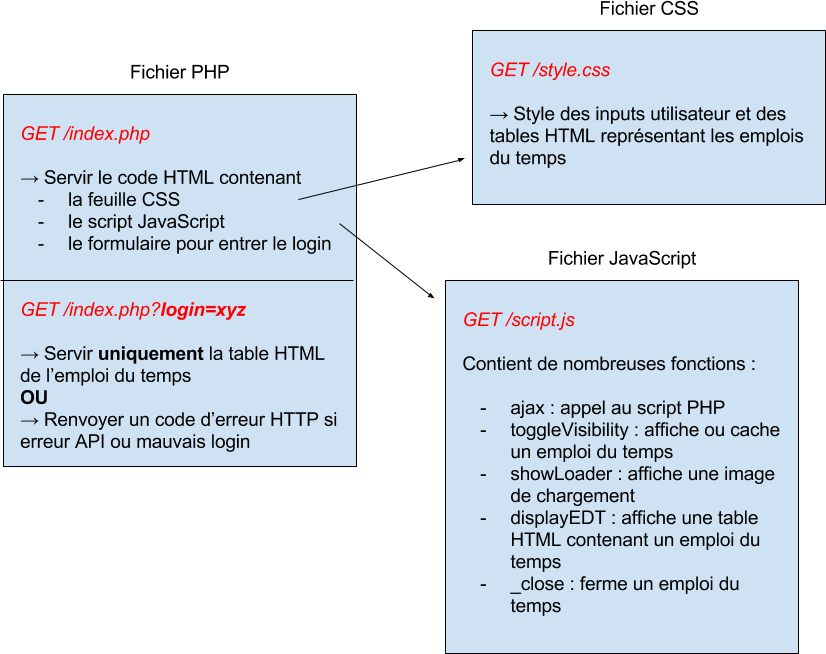
\includegraphics[width=1.00\textwidth]{images/arch.png}
    \caption{Architecture du projet}
\end{figure}

Le JavaScript fera un appel à notre fichier PHP pour récupérer l'emploi du temps d'un étudiant, en transmettant dans la requête son \textit{login}. La réponse contient directement du code HTML qui sera ``inclu'' dans notre page actuellement affichée grâce à JavaScript. Il y a quelques éléments visuels de \textit{feedback} (mauvais \textit{login}, API indisponible, etc).

\medskip

Le code PHP, à la réception d'une requête HTTP contenant un paramètre \lstinline{GET} nommé \lstinline{login}, va aller faire une requête sur l'API de l'UTC\footnote{\url{https://webapplis.utc.fr/Edt_ent_rest/myedt/result?login=<login>}} afin de récupérer l'emploi du temps correspondant au \textit{login}. Cet emploi du temps, servi sous le format JSON, va être traité par notre code PHP afin d'obtenir en résultat final une \lstinline{<table>} HTML. Le code PHP va envoyer ce code HTML final en réponse à la requête envoyée par le JavaScript.

\medskip

Le JavaScript va inclure directement dans la page la table HTML reçue en réponse. Ainsi, il nous est très facile d'afficher plusieurs emplois du temps les uns à la suite des autres. Chaque requête avec un \textit{login} nous permet de récuperer un table HTML qu'il nous suffit de rajouter à la suite, dans notre page couramment affichée.

\section{Résultat final}

\begin{figure}[H]
    \centering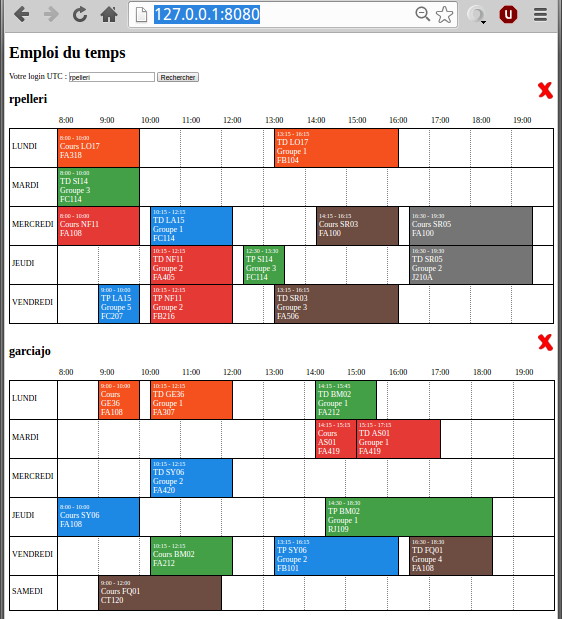
\includegraphics[width=1.00\textwidth]{images/edt.png}
    \caption{Emplois du temps}
\end{figure}

\section{Fonctionnalités ajoutées}

\begin{itemize}
  \item Message d'erreur affiché si l'API de l'UTC ne répond pas un code 200
  \item Message d'erreur si mauvais login entré (l'API de l'UTC rendra un tableau JSON vide)
  \item Possibilité d'afficher plusieurs emplois du temps
  \item Possibilité de cacher temporairement des emplois du temps en cliquant sur le login (accordéon)
  \item Possibilité de fermer un emploi du temps ouvert définitivement
  \item Vérification que l'utilisateur n'essaie pas d'afficher deux fois le même emploi du temps ou qu'il ne valide pas le formulaire sans avoir rempli le champ pour le \textit{login}
  \item Affichage du samedi que s'il y a un créneau horaire occupé
  \item Affichage d'une image de chargement (\textit{loader}) en attendant la réponse de notre script PHP suite à l'envoi d'un \textit{login}
\end{itemize}

\section{Difficultés rencontrées}

La grosse et unique difficulté a été la création de la table HTML servant à afficher un emploi du temps. Pour construire une \lstinline{<table></table>} il faut procéder ligne par ligne (\lstinline{<tr>...</tr>}) d'où notre choix d'affichage des jours les uns au-dessus des autres. Un petit algorithme a pour cela été mis en place (un autre également pour trier par jour et heure les cours, à partir du JSON reçu par l'API de l'UTC).

\section{Comment exécuter le projet}

\fakeshell
\begin{lstlisting}
sudo apt-get install php5-cli # Ou installer php5-cli avec un autre package manager, en fonction de l'OS utilisé

cd code/ # Aller dans le dossier contenant le code source
php -S 127.0.0.1:80 -t .
\end{lstlisting}
Puis ouvrir un navigateur Web et aller à \url{http://127.0.0.1:8080}.
